\documentclass[internal]{FRIreport}

% AMS fonts required
\usepackage{iopams}  
\usepackage{float}

% package to include graphics in ps, eps or png format
\usepackage{graphicx}
% the graphics path
\graphicspath{{img/}}

% define equation referencing
\newcommand{\eqref}[1]{(\ref{#1})}

% define figure referencing
\newcommand{\figref}[1]{Fig.~\ref{#1}}

% define real numbers symbol
\newcommand{\Rset}{\ensuremath{\mathbb{R}}} 
\newcommand{\R}{\Rset} 
% define natural numbers symbol
\newcommand{\Nset}{\ensuremath{\mathbb{N}}} 
\newcommand{\N}{\Nset} 
% define euclidean vector space symbol
\newcommand{\Eset}{\ensuremath{\mathbb{E}}} 
\newcommand{\E}{\Eset} 

\newcommand{\imp}[1]{{\color{P654M}#1\normalcolor}}

%main
\begin{document}



\title{Influence of predator/prey endurance on predator evolution}

\author[ \etal]{Veronika Blažič, Nataša Hribar, Tanja Štular, Manca Žerovnik}

\address{University of Ljubljana, Faculty of Computer and Information Science, Ljubljana, Slovenia}

\begin{abstract}
We implemented endurance into the evolution model of predator attack tactics when attacking fish achools. Taking into consideration prey and predator energy consumption attacking the peripheral prey (as opposed to attacking the nearest prey in simulations without endurance implementation) is revealed as the optimal attack tactic. 

\Keywords{fish fatigue, endurance, fish schools, artificial life, prey, predator, attack tactics, evolution model, simulation}
\end{abstract}



%
%%
\section{Introduction}
%
%%Intro %%%
Our work focuses on evolution of predator attack tactics when attacking fish schools. In the model developed by Demsar et al. \cite{demvsar2015simulating} predators and prey have infinite energy, meaning that they can move at their maximum speed for as long as they want. In nature, however, this is obviously not the case, an animal can move at a maximum speed only for a certain amount of time before it gets fatigued. In this project we will try to implement endurance into our model and analyze how it influences the result of the evolution.
~\\\\
In previous studies the biological experiments were made to gain data about fish endurance. In 1959 Bainbridge \cite{bainbridge1960speed} observed three different species of fish. He discovered that there are two speed values that are especially important. First one is the maximum speed a fish can achieve, but the maximum speed can only be maintained for a very short period of time. The other important speed is the cruising speed, which is a lower speed that a fish can sustain for longer periods of time. In order to reach the maximum speed a fish uses most of its energy, so it can only maintain this speed for a very short time of 1-2 seconds. After that, it starts rapidly losing its velocity, until its current speed is almost the same as its cruising speed. \\
Figure \ref{ref:graf1} shows the relationship between speed and time for seven different daces of different lengths that were obtained by Bainbridge's experiments. We can see the speeds quickly converge to their cruising speeds of 80-90 cm/s. 
\begin{figure}[htb]
\label{ref:graf1}
\centering
\includegraphics[scale=0.9]{1.png}
\caption{Relationship between speed and time observed in seven different daces of different lengths.}
\end{figure} \hfill \break
The fish eventually looses all of its energy and it's forced to stop in order to regenerate. The maximum distance a fish can swim depends on its body length, meaning longer fish can swim greater distances before needing to stop. Figure \ref{ref:slika2} illustrates the maximum distance hypothetical fish of four different body lengths can travel.
\begin{figure}[H]
\centering
\includegraphics[scale=0.9]{2.png}
\caption{Maximum distance, speed and fish length.}
\label{ref:slika2}
\end{figure} \hfill \break
The recovery happens if the fish is resting. It recovers 31\% of it's energy in first hour, 42\% of energy after 2 hours, 67\% after 3 hours, but reaches full recovery of 100\% after 18-24 hours.
~\\\\
Videler and Wardle \cite{videler1991fish} researched how swimming characteristics relate to reproduction, food capture and escaping from predators. They used four different methods to get the data for observing speed limits and endurance of swimming fish. They discovered that speed and also endurance differ among species. Tail beat frequency was exposed as the most important feature when modulating speed. Their results showed that swimming characteristics are also related to the water temperature, since the maximum speed doubles with every 10 degrees. Endurance between individuals differs for 25\% in same species. Larger fish can swim at higher absolute speed and for every species the curve of endurance is very different. Similarity between fish with shallow endurance curve was found: they are usually small and are not pelagic long-distance swimmers.
~\\
%%% Pelaške ribe, dalmatinsko in pogovorno primorsko plava riba, so ribe, ki živijo v jatah na odprtem morju do srednjih globin. Njihovo meso je temnejše barve, ker so te ribe izraziti plavalci. Veliko pelaških ribjih vrst je roparskih.%%%
~\\
The energy control in a predator-prey model has been represented by Lee in 2013 \cite{lee2013evaluation}. Lee simplified the simulations by using only one predator and prey and also by removing the obstacles from the environment. Predator attacked when it had enough energy and when the predator attacked, prey ran away with its maximum force. Forces can be described as seek and flee forces. For both predator and prey mass, location, velocity, and acceleration were taken into account for energy calculations. When predator was chasing its prey target, both predator and prey had to spend energy in order to reach their maximum velocities.\\\\
Energy was calculated as: \\
\begin{equation} \label{eq:energy}
E_{c}(i,j) = \sum\limits_{k=1}^n [ f_{p}(i,j, \Delta t_{k}) + m_{i} \mu  ] f_{ \Delta t_{k}}, 
\end{equation}
where $f_{ \Delta t_{k}}$ is the distance to move during time $\Delta t_{k}$ and it can be computed with acceleration known from the force $f_{p}(i,j, \Delta t_{k})$.

%\begin{equation} \label{eq:seekp}
%f_{p}(i,j, \Delta t) = f_{s} (i, p_{j} + v_{j} x t, \delta t)
%\end{equation}
%\begin{equation} \label{eq:seek}
%f_{s}(i,j, \Delta t_{k}) = m_{i} \frac{(p-p_{i}).norm() * v_{mi} - v_{i}}{\Delta t}
%\end{equation} \hfill \break \break

\section{Methods}

\subsection{Model Introduction} \label{sssec:tactics}
For the basis of our work we upgraded the model developed Demsar et al. \cite{demvsar2015simulating} In this model the predators use two types of tactics: \\
\begin{itemize}
\item Predators that in successive attacks based on probability choose one of several simple attack tactics  (in model we use three simple attack tactics: attack nearest prey, attack central prey, attack peripheral prey).\\
\item Predators that first disperse prey and then pick isolated individuals. Predator agent adapts its probability that a specific tactic will be selected in next attack, the distance at which it stops dispersing the prey and the radius within it searches for the most isolated prey.
\end{itemize}
~\\
Prey can move in two different settings:\\
\begin{itemize}
\item A delayed response is efficient prey defence tactic, for example fish schools often delays its escape response to a later point in time and then tries to outsmart the predator with rapid movements.\\
\item Predator confusion plays important role in the evolution of composite tactics\\
\end{itemize}
\textbf{Model}
Our model is for computational simplicity two-dimensional. It consists of two types of agents -- a solitary predator and group of prey. The goal of prey is to survive, while the predator tries to catch as many prey individuals as possible. In our model the behavior of prey is not the part of the evolutionary process it is pre-set so that the group of prey moves in a polarized cohesive manner; only the behavior of predator evolves. Predator is set to be 1.5 times faster than the prey, but it is also less manoeuvrable. In the simulations, where predator had the same speed as prey, it almost never caught it.\\

%\textbf{Prey}\\

%The mechanism of neighbourhood perception is vision. Field of view is 300 degrees with a blind angle of 60 degrees behind it. Field of view consist of N agents that are:
%\begin{itemize}
%\item	not the observed itself\\
%\item	within the 300 degree visual range\\
%\end{itemize}
%\begin{equation} 
%N = {j \epsilon A, j \neq  i, \overrightarrow{v} * \overrightarrow{d}_{j}  \geq  \upsilon} \end{equation}
%A: set of consisting of the predator and prey agents \\
%I: observed prey agent \\
%\overrightarrow{v}: current velocity
%\begin{equation}\upsilon = \overrightarrow{v} / \| \overrightarrow{v} \|\end{equation}: current heading\\
%\begin{equation} \overrightarrow{d} = ( \overrightarrow{p} - \overrightarrow{p} ) / \| \overrightarrow{p} - \overrightarrow{p} \| \end{equation}: the unit direction vector pointing from the current position of the observed prey agent to the current position of agent  and  is the cosine of the prey’s field of view. 

%A prey agent has four drives and thus four zones – separation, alignment, cohesion, and escape zone.
%Each of the four drives returns an acceleration vector that represents the prey’s action according to the specific drive. The actual acceleration that is used to update the prey’s velocity, is calculated as a weighted sum of all four drives: 
%\begin{equation} 
%\overrightarrow{a} = w_{s}\overrightarrow{a}_{s} + w_{a}\overrightarrow{a}_{a} + w_{c}\overrightarrow{a}_{c} + w_{e}\overrightarrow{a}_{e}
%\end{equation}
%Prey’s cruising and maximum speed: 
%\begin{equation} 
%\overrightarrow{v}' = \left [ \overrightarrow{v} + \left [ \overrightarrow{a}_{0, a_{m}}\Delta t \right ]  \right ] : current velocity of the observed prey agent 
%\overrightarrow{p}' = \overrightarrow{p} + \overrightarrow{v}' \Delta t : current position
%a_{m} and v_{m} : the prey’s maximum acceleration and maximum speed, 
%v_{c}: the prey’s cruising speed, 
%\Delta t: the simulation time step,
%\overrightarrow{v} and \overrightarrow{p} : the velocity and position of the observed prey agent in the next simulation time step respectively.
%\end{equation}
%%mogoce dodaj se enacbe (natasa)
%The three drives, separation, alignment, and cohesion, are the drives that are most commonly used in computer models of collective behaviour (Reynolds 1987). 
%The escape drive represents the prey’s tendency to escape from the predator. It is represented as the acceleration away from the predator’s current position. 
%The maximum speed of prey was set to 4 BL/s, and the cruising speed was set to 2 BL/s. Zone sizes and zone weights were set in a way that when prey was not under the threat of predation, prey moved in a synchronized cohesive manner while maintaining an inter-individual distance of 1-2 body.
%\textbf{Predator} \\
%View in our model is 360 degrees wide – there is no blind angle. Agent can perceive prey in a radius of 400 BL.
%Behaviour of the predator is governed only by the hunt drive; the hunt drive is defined as an acceleration that points towards the position of the current target which depends on the predator’s.
%\begin{equation} 
%\overrightarrow{v}' = \left [ \overrightarrow{v} + \overrightarrow{a}_{h} \Delta t  \right ]_{\left [ v_{cp'}, v_{mp} \right ]}
%\end{equation}

%\begin{figure}[htb]
%\includegraphics{Table_1.png}
%\caption{Values and parameters that are used in our model.}
%\label{parameters}
%\end{figure}

%\textbf{Experiments}\\
%Described in two phases:
%\begin{itemize}
%\item the evaluation phase\\
%\item the evolution phase\\
%\end{itemize}
%Once the current generation of predators completed their runs, the evaluation phase finished and the evolution phase began.
%Default values for the mutation rate, mutation factor and other genetic algorithm parameters are given in table 2.

%\begin{figure}[htb]
%\includegraphics{Table_2.png}
%\caption{Values and parameters in experiment.}
%\label{parameters}
%\end{figure}

%The probability that this attempt was successful was inversely proportional to the number of individuals within the predator’s confusability zone.

%The target selection process was repeated every time a) the predator’s attempt to catch the targeted prey was unsuccessful and the refocus time passed, or b) the predator caught the targeted prey and the handling time passed. That means that the predator could use different simple tactics on successive attacks during one simulation run (600 time steps). In the evolution phase the chromosome of a new predator (offspring) was generated by using the coin-flip crossover, a type of crossover operator that chooses a gene from one of the parents at random (uniform distribution). The coin-flip crossover was repeated for all genes. Occasionally, being governed by the mutation rate (2 \% per parameter), the genes mutated. The mutation of a specific gene, i.e. probability of a specific tactic, was simulated as either an increase or a decrease (chosen at random) of the likelihood that the predator will use that particular tactic. The amount of increase/decrease was governed by the mutation factor (20 \%). Because the cross-over and mutation could lead to the sum of probabilities not being equal to 1, the last step in the creation of a new chromosome was renormalization, i.e. division of individual probabilities by their sum. 

%%spremeni v eps
%\begin{figure}[htb]
%\includegraphics{Table_3.png}
%\caption{Evaluation parameters.}
%\label{parameters}
%\end{figure}

%%%% konec natasa

\subsection{Endurance Implementation}
For the implementation of endurance we found multiple potential methods that consider previous biological studies. In the following subsections the detailed introduction of our method will be represented.


\subsubsection{Method Description}
The idea for this method originates from the research conducted by Plaut \cite{plaut2001critical}. The main idea is that fish have three different speed modes - sustained mode, burst mode and prolonged mode. Referring to biological studies, we set a time interval for each mode. The time interval determines for how long a fish can be in one particular mode. Depending on the speed, the energy of the fish either increases, decreases, or stays the same. During a predator attack, an ideal flee force is calculated. The ideal flee force is the one which makes the prey advance away from the predator with maximum acceleration \cite{lee2013evaluation}. The acceleration is reduced (if necessary) due to available amount of energy that prey contains. If the prey lacks energy, the velocity slowly decreases, until it reaches the highest value which the fish can retain for a certain amount of time without getting tired. As Fish explained in 2010 \cite{fish2010swimming}, the endurance of the fish also depends on its position in the school. We assume that the fish in the leading position needs to spend more energy to retain its speed than the fish positioned after it.
~\\
\subsubsection{Implementation - Prey}
We set the starting speed of prey to two body lengths per second. The starter timer, which represents normalized conserved energy, is set to 1. Every second the fish energy changes due to speed it currently swims with. From the equation 
~\\
\begin{equation} \label{eq:energy3}
E_{consumed} = 1324.83 * e^{-0.047259 * v},
\end{equation}
~\\
where \textit{v} 
represents the current speed, we calculate an energy weight, which inverse and normalized value is deducted from the timer. Equation \ref{eq:energy3} is inverse function of 
~\\
\begin{equation} \label{eq:energy4}
time(v) = -21.16*ln(v) + 152.12
\end{equation}
~\\
which represents ratio between speed and the longest time interval the fish can swim with corresponding velocity before it loses all its energy. Function was calculated from the experimental data measured in past research. Also if a fish is in the leading position we increase its energy loss. Every second when fish speed is calculated we check if the timer is bigger than zero then there is no effect on the speed or acceleration, 
the fish has enough energy stored. In the opposite case, the prey's speed changes to prolonged mode, which in our case equals to two times its body length per second. While the prey is in prolonged speed mode its timer increase every second by $\frac{1}{prey size * 150}$ which represents energy regeneration.
~\\\\
\subsubsection{Implementation - Predator}
Predator's endurance implementation is similar to prey's. Its energy is decreasing or increasing due to the speed it currently swims with. Through evolution, the predator is learning how much energy it needs to successfully complete the pursuit and will only start to pursuit the prey, if it has enough energy to reach it. In the start the energy threshold is chosen randomly between 0.1 and 0.9. When starting the attack, the predator speeds up to its turbo speed (10 body lengths per second). In order to reach the turbo speed, it needs to have at least 50\% of its starting energy, if not the predator goes to prolonged speed mode in which it regenerates its energy and then continues with the pursuit of the prey. 

%preverja energijo in razdaljo, in se -> prag == se uči; in distance; začetna je random med 0.1 in 0.9; distance med catch distance*4 in *6; plen ma 1.5 sustained speed; velikost iz 6 na 4; ker je bil prevelik in prehitr _> premalo okreten; regGain
%framesToGetRecovered = AppSettings::predatorSize * 150; //fish is completly regenerated
%  regenerationGain = 1 / (framesToGetRecovered); // canturbospeed, ko ga uporabi prvič mora nazaj sšet nafilat energijo na 0.5; v turbo mode gre ko je v bližini ribe (se nauči to kdaj); v jati je vsaka riba drugače velika -> izbira drugo taktiko :))))))

\section {Results}
We ran the simulations on both types of predator tactics described in \ref{sssec:tactics}. We stopped each evolutionary run after 400 generations and repeated the whole process 10 times. Number of flocks was set to 5 while number of frames per generation was 600. Predator size was modified from 2 to 4 also prey sizes were changed to randomly generated numbers from 0.7 to 1.3.  
\subsection{Simple tactics}
Figure \ref{ref:results1} visualizes the average number of prey, that the predator caught through generations. The predator was more successful in the simulation without fatigue implementation. Figure \ref{ref:results2} represents predator and prey distance, when the predator entered the turbo speed mode. The ideal distance, at which the predator starts the attack and enters turbo mode, was part of the evolutionary process. Distance threshold is connected with the energy threshold, which tells us how much energy the predator needs for a successful attack. In figure \ref{ref:results3} we can see how this threshold is changing and also that distance threshold affects hunt count since they converge at the same time.\\
Another property that we observed were the tactics that the predator used for selecting its target. As described in the subsection \ref{sssec:tactics}, the predator can choose from three different tactics: attacking the nearest prey, attacking the central prey or attacking the peripheral prey. In figure \ref{ref:results4} the probabilities of choosing each of the tactics are shown both for the implementation with fatigue and the implementation without it.  When we added fatigue, the evolved predator preferred to target the nearest prey and without fatigue, the evolved predator preferred to target the most peripheral prey. We can explain change of the chosen tactic by predators awareness of its energy limitation. The predator obviously do not have enough energy to successfully attack the peripheral prey so it begins to pursuit the nearest prey. Consequently the number of hunted prey is higher which is also associated with the non-evolving prey. 
 
\begin{figure}[H]
\centering
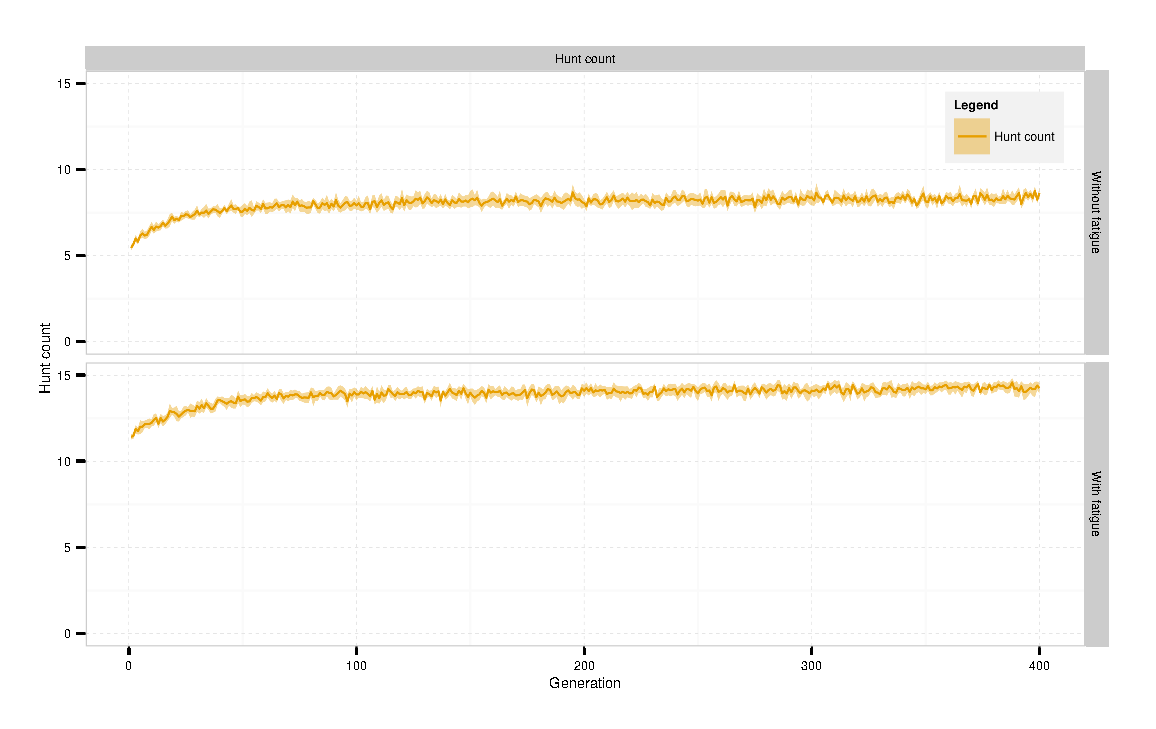
\includegraphics[scale=0.7]{hunt_success.eps}
\caption{Comparison of average numbers of prey that predator caught in a single evolutionary run for both implementations (with and without endurance).}
\label{ref:results1}
\end{figure} \hfill 

\begin{figure}[H]
\centering
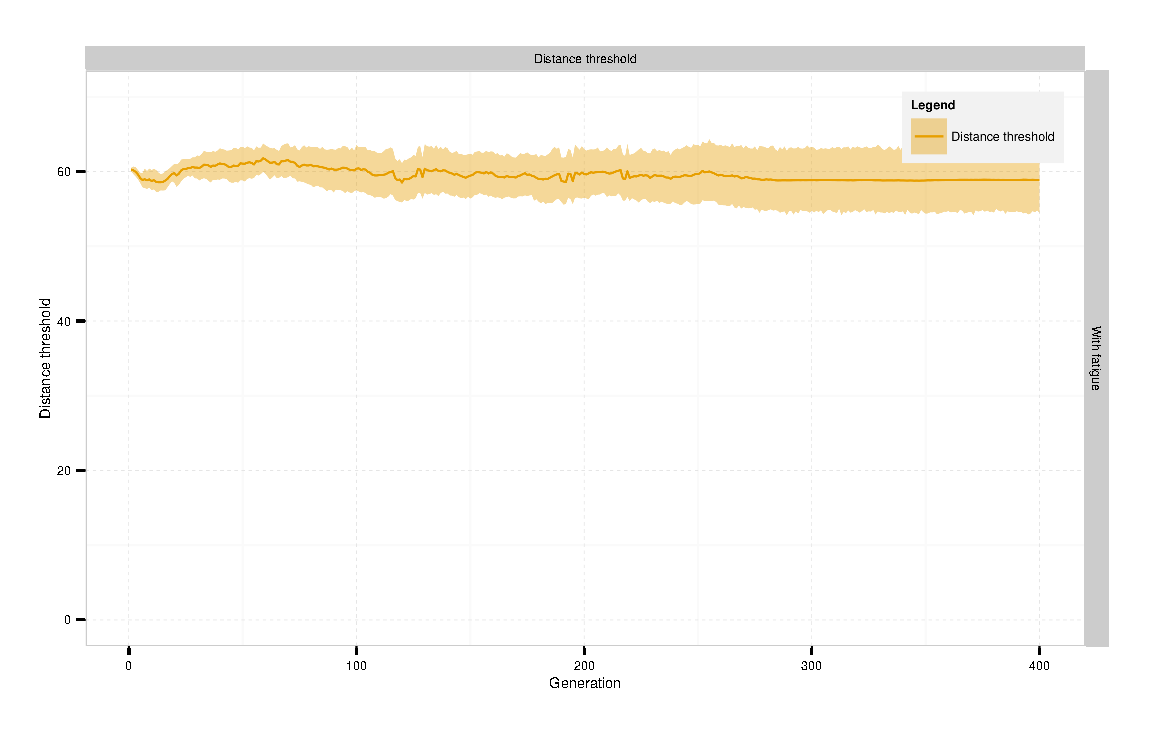
\includegraphics[scale=0.7]{distance_graph.eps}
\caption{Distance between predator and prey when predator activates turbo speed.}
\label{ref:results2}
\end{figure} \hfill

\begin{figure}[H]
\centering
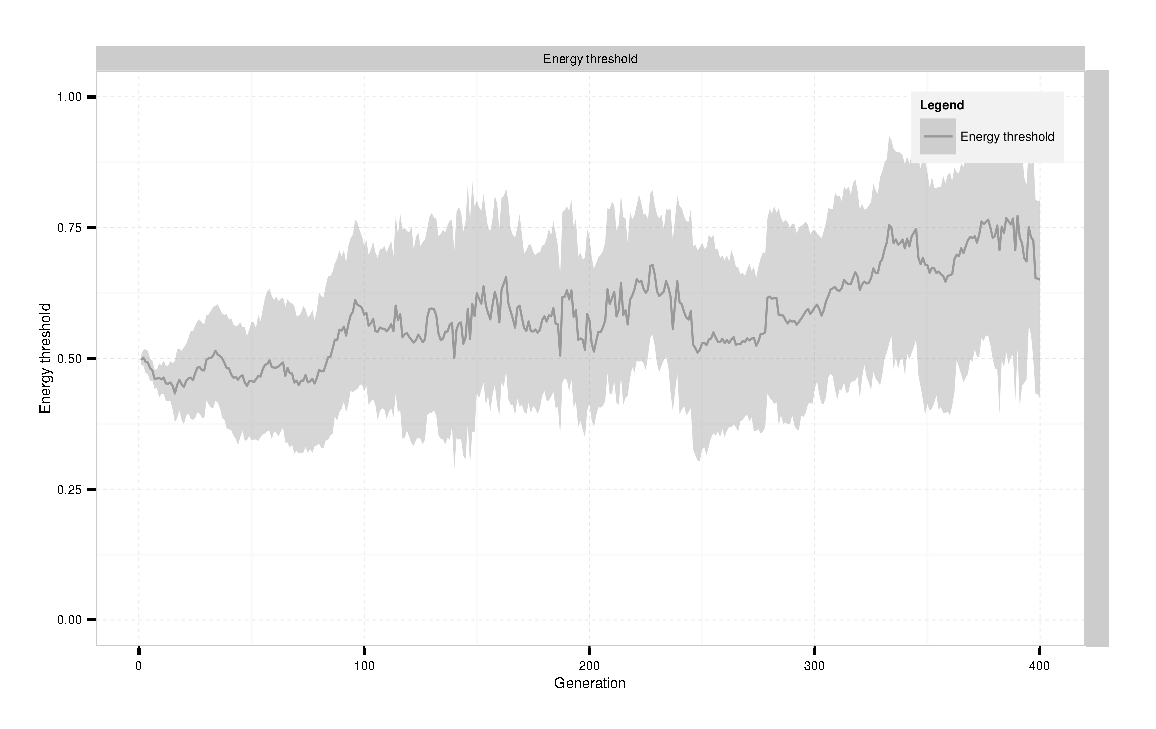
\includegraphics[scale=0.7]{energy_graph.eps}
\caption{Energy threshold to start an attack in single generation.}
\label{ref:results3}
\end{figure} \hfill 

\begin{figure}[H]
\centering
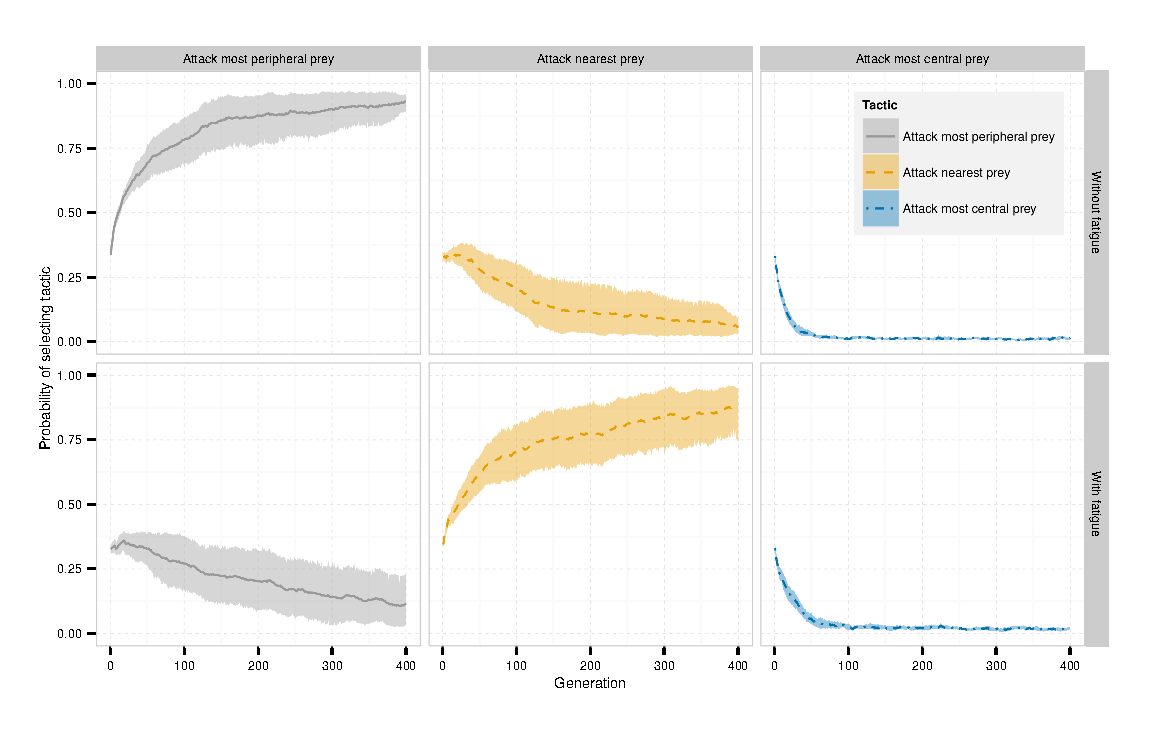
\includegraphics[scale=0.75]{tactics_graph.eps}
\caption{Comparison of probabilities that certain tactic will be chosen in a single generation in simulations with and without endurance implementation.}
\label{ref:results4}
\end{figure} \hfill 
\subsection{Disperse tactic}
We have also observed the predators behavior with disperse tactic. Obtained results for number of hunted prey (figure \ref{ref:results5}) were similar as before. On figure \ref{ref:results6} we can see how the distance at which predator stops dispersing the prey (lock on distance) and the radius within it searches for the most isolated prey (lock on radius) have changed with implementation of fatigue. The lock on radius did not change significantly but lock on distance scaled down which means that now predator attacks earlier.

\begin{figure}[H]
\centering
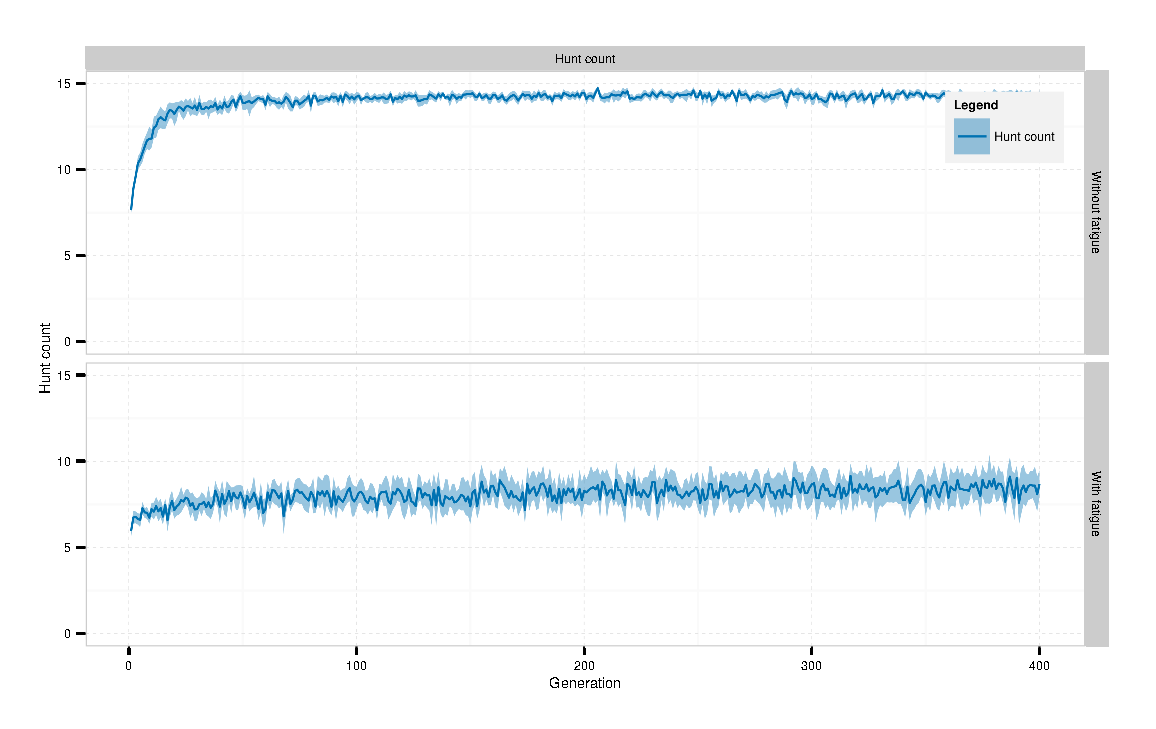
\includegraphics[scale=0.75]{dispersehuntcount.eps}
\caption{Comparison of probabilities that certain tactic will be chosen in a single generation in simulations with and without endurance implementation.}
\label{ref:results5}
\end{figure} \hfill 
\begin{figure}[H]
\centering
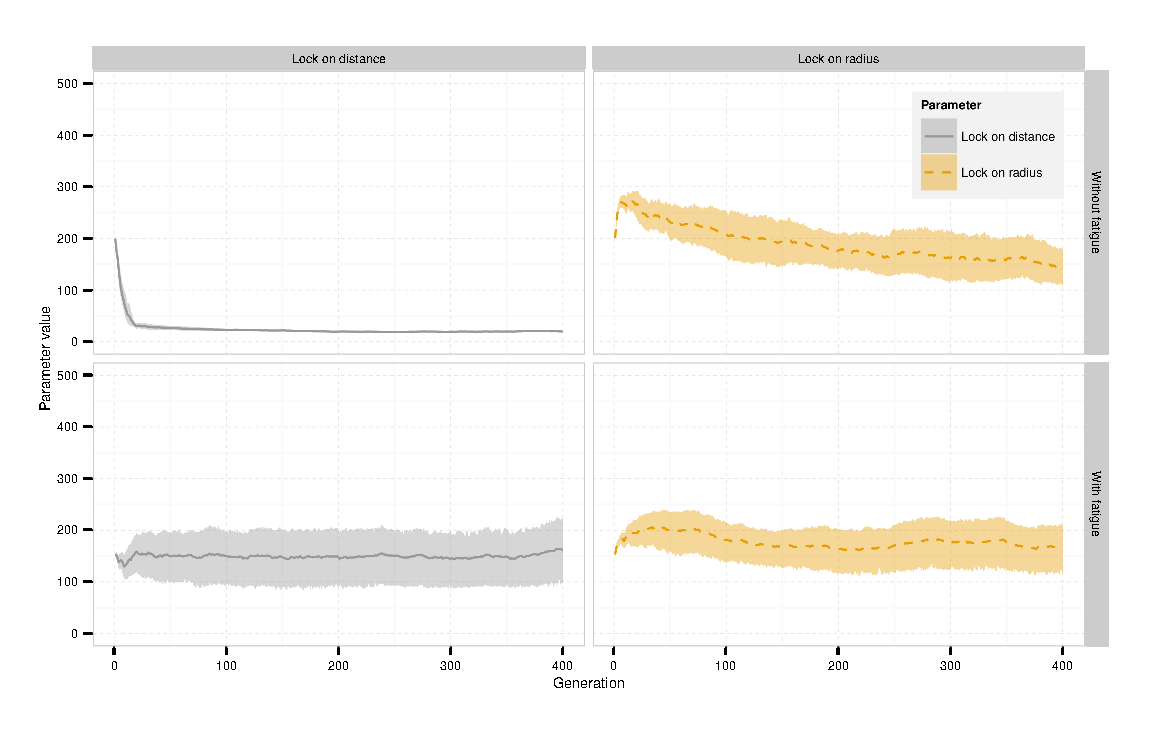
\includegraphics[scale=0.75]{disperse_graph.eps}
\caption{Comparison of probabilities that certain tactic will be chosen in a single generation in simulations with and without endurance implementation.}
\label{ref:results6}
\end{figure} \hfill 
%dispersing slika je bil torej poskus k smo opazovali plenilca ki je ves čas napadal z razprsitveno taktiko (dispersing tactic) opazovali pa smo razdaljo do centra najbližje skupine, ki nam pove kdaj bo nehal loviti srednjega in se osredotočil na robnega. Tam pa imamo se radij ki nam pove v kakšnem radiju išče najbolj robnega.

%
%%
%\section{Results and Discussion}
%

%
%%
\section{Conclusion}
We focused on implementing prey and predator endurance in evolution of predator attack tactics, when attacking fish schools. It was taken in account, that fish can swim in three speed modes - sustained mode, burst mode and prolonged mode. In correspondence with these modes, fish energy either increases or decreases every second. The average number of prey, that the predator caught through generations, was higher in simulations with the endurance implementation, meaning the predator was now more successful than in simulations without endurance. Predator learned through generations the ideal attack tactic and energy threshold, needed to catch the prey. The probability that certain tactic will be chosen is different to the probability in simulation without fatigue. In latter, the predator chose the 'attack the most peripheral prey' tactic, while in our model, it chose the 'attack the nearest prey' tactic. In disperse tactic simulation the distance at which predator stops dispersing the prey scaled down when the fatigue is taken in account. 
~\\\\
Because it is not natural that only predator evolves for future work we propose similar implementation also for the prey. The latter could significantly change the results. Also the biological assistance should be derived for making initial parameters more accurate. 
%
%finish by giving a concise explanation of the obtained results and eventual future research directions

%
%%
\section*{Author contributions}
%
All authors contributed equally to this work.
%
%%
\pagebreak
\References
%
\bibliographystyle{elsart-num}
\bibliography{ilb_bibliography,qdCAD_bibliography}

\end{document}